\documentclass[10pt, a4paper, spanish]{article}
\usepackage[paper=a4paper, left=1.5cm, right=1.5cm, bottom=1.5cm, top=3.5cm]{geometry}
\usepackage[spanish]{babel}
\selectlanguage{spanish}
\usepackage[utf8]{inputenc}
\usepackage[T1]{fontenc}
\usepackage{indentfirst}
\usepackage{fancyhdr}
\usepackage{latexsym}
\usepackage{lastpage}
\usepackage[colorlinks=true, linkcolor=blue]{hyperref}

\usepackage{listings}
\lstset{language=C++,
		basicstyle=\ttfamily}

\usepackage[Algoritmo]{algorithm}
\usepackage{algpseudocode}
\algrenewcommand\textproc{}% Used to be \textsc Para que el nombre de la función no sea en mayusculas

\usepackage{tabularx} % tablas copadas
% \usepackage{graphicx}
\usepackage{amsmath, amsthm, amssymb}

%\usepackage{makeidx}
\usepackage{paralist} %itemize inline
\usepackage[table]{xcolor}
\usepackage{caratula/caratula}

\usepackage{float}
\usepackage{amsfonts}
\usepackage{sectsty}
\usepackage{charter}
\usepackage{wrapfig}

\usepackage{caption}
%el de arriba funciona si no esta, el de abajo quite el "Figura #" de las imagenes
\captionsetup[figure]{labelformat=empty}

\begin{document}

\titulo{Trabajo práctico I}

\subtitulo{Scheduling}

\materia{Sistemas Operativos}

\integrante{Cámera, Joel Esteban}{257/14}{joel.e.camera@gmail.com}
\integrante{Lavia, Alejandro Norberto}{43/11}{lavia.alejandro@gmail.com}
\integrante{Guttman, Martín David}{686/14}{}


\maketitle

\tableofcontents

\newpage
\section{Ejercicio 1}

Para la resolución de este ejercicio, se requeria programar un tipo de tarea \emph{TaskConsola} donde debia realizar $n$ llamadas bloqueantes, cada una con una duración aleatoria de valor $random\_num: bmin \leq random\_ num \leq bmax$.
~
Para lograr esto, ciclamos \emph{n} veces en el cual, en cada iteración generamos un número pseudoaleatorio utilizando la función \textbf{rand()} de la forma:

\begin{center}
	\textbf{random\_num = bmin + rand() \% (bmax - bmin + 1)}
\end{center}

Una vez hecho esto, realizamos la llamada bloqueante con la cantidad de clocks definida por ese valor pseudoaleatorio creado y luego ejecutamos un clock.

\begin{figure}[!h]
	\begin{center}
		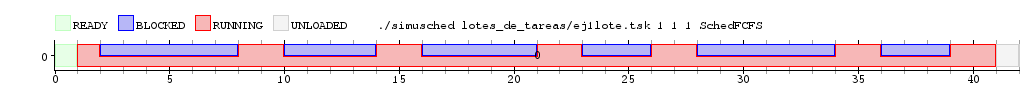
\includegraphics[width=500px]{imagenes/ej1.png}
		\caption{\emph{TaskConsola} corriendo con $n = 6$, $bmin = 3$ y $bmax = 7$.}
	\end{center}
\end{figure}

\newpage
\section{Ejercicio 2}

Para este ejercicio se pedía ejecutar y graficar usando el algoritmo \textbf{FCFS} para 1, 2 y 4 núcleos, con un cambio de contexto de 2 ciclos, para la tarea (\emph{ej2lote}): 

\begin{center}
	\begin{tabular}{|l|}
		\hline
		TaskCPU 10			\\
		@5:					\\
		TaskConsola 5 1 4	\\
		@6:					\\
		TaskConsola 5 1 2	\\
		@8:					\\
		TaskCPU 10			\\
		\hline
	\end{tabular}
\end{center}

Los graficos en cuestión son:

\begin{figure}[!h]
	\begin{center}
		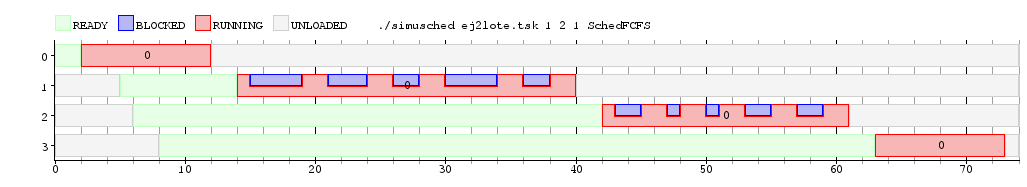
\includegraphics[width=500px]{imagenes/ej2_1.png}
		\caption{Ejecución del lote \emph{ej2lote} con 1 núcleo.}
		\label{fig:grafico_ej2_1}
	\end{center}
\end{figure}

\begin{figure}[!h]
	\begin{center}
		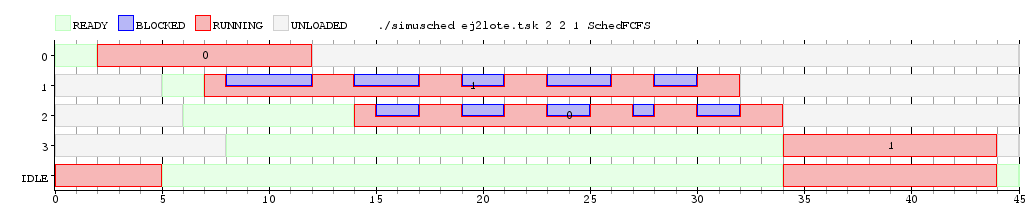
\includegraphics[width=500px]{imagenes/ej2_2.png}
		\caption{Ejecución del lote \emph{ej2lote} con 2 núcleos.}
		\label{fig:grafico_ej2_2}
	\end{center}
\end{figure}

\begin{figure}[!h]
	\begin{center}
		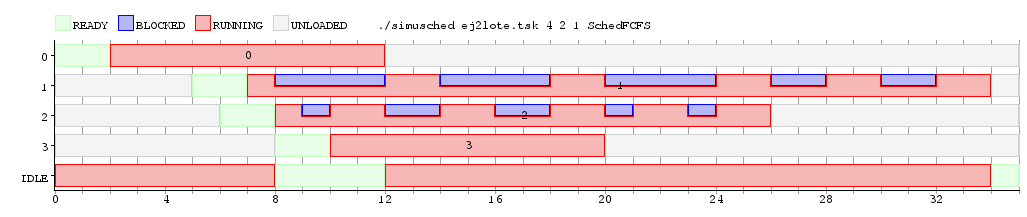
\includegraphics[width=500px]{imagenes/ej2_4.png}
		\caption{Ejecución del lote \emph{ej2lote} con 4 núcleos.}
		\label{fig:grafico_ej2_4}
	\end{center}
\end{figure}

\newpage
Realizamos el calculo de la \textit{latencia}:

\begin{center}
	\begin{tabular}{|c|c|c|c|c|}
		\hline
		\multicolumn{5}{|c|}{\textbf{Latencia}} \\
		\hline
		\textbf{Cant. Nucleos} & \textbf{TaskCPU @0} & \textbf{TaskConsola @5} & \textbf{TaskConsola @6} & \textbf{TaskCPU @8} \\
		\hline
		1 & 2 & 9 & 36 & 55 \\
		2 & 2 & 2 & 8 & 26 \\
		4 & 2 & 2 & 2 & 2 \\
		\hline
	\end{tabular}
\end{center}

\textit{Throughput} obtenido (rendimiento, expresado en cantidad de procesos terminados por unidad de tiempo):
\begin{figure}[!h]
	\begin{center}
		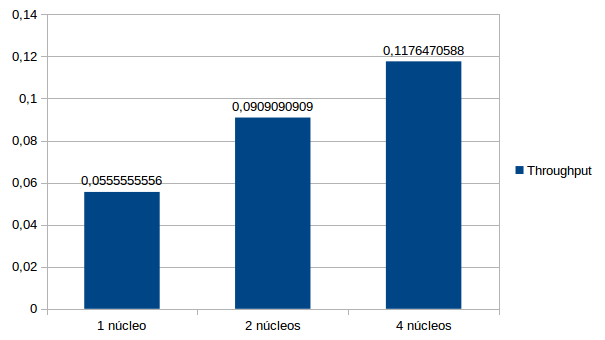
\includegraphics[width=250px]{imagenes/ej2_throughput.png}

		\label{fig:grafico_ej2_throughput}
	\end{center}
\end{figure}

Como se puede observar en el gráfico, el throughput se incrementa a medida de que aumenta la cantidad de núcleos.


\newpage
\section{Ejercicio 3}

En este ejercicio nos piden programar la tarea \textbf{TaskBach} que recibe dos parámetros: \textit{total\_cpu} y \textit{cant\_bloqueos}. La misma debe realizar \textit{cant\_bloqueos} llamadas bloqueantes en momentos elegidos pseudo aleatoriamente y, en cada una de esas llamadas debe permanecer bloqueada durante dos ciclos de reloj. El tiempo de CPU total utilizado debe ser el de \textit{total\_cpu} ciclos de reloj.

Para que esta tarea tenga el comportamiento pedido, lo que hacemos contar cual es la cantidad de tiempo que se va a utilizar el CPU de la siguiente forma:

\begin{center}
		int \textit{cpu\_restante} = \textit{total\_cpu} - \textit{cant\_bloqueos} - 1;
\end{center}

Cada llamada bloqueante utiliza un ciclo de reloj y la función \textbf{return} también utiliza un ciclo. Por ende, los ciclos restantes son los que utilizamos para hacer la llamada a la función \textbf{uso\_CPU}.

Luego, tenemos el siguiente ciclo:

\begin{algorithmic}

\While{\emph{cant\_bloqueos}$> 0$}
	\State Genero un número pseudoaleatorio entre cero y \textit{cpu\_restante} con la función \textbf{rand()}.
	\If{\emph{Si el número generado es mayor que cero}}
		\State Utilizo el CPU ese número generado de clocks.
	\EndIf
	\State Le resto a \textit{cpu\_restante} el número generado.
	\State Llamo a la función \textbf{uso\_IO} con dos clocks.
	\State Le resto uno a \textit{cant\_bloqueos}
\EndWhile
\end{algorithmic}
~
De esta forma, vamos a obtener llamadas bloqueantes en momentos elegidos pseudo aleatoriamente.

Generamos y ejecutamos el siguiente lote, y luego graficamos la simulación usando el algoritmo FCFS con un costo de 3 clocks para cambiar de contexto.

\begin{center}
	\begin{tabular}{|l|}
		\hline
		TaskBatch 23 1		\\
		@5: 				\\
		TaskBatch 42 2		\\
		@6:					\\
		TaskBatch 58 3		\\
		@8:					\\
		TaskBatch 77 4		\\
							\\
		TaskBatch 33 12		\\
		@2:					\\
		TaskBatch 50 5		\\
		@3:					\\
		TaskBatch 70 9		\\
		@2:					\\
		TaskBatch 27 3		\\
		\hline
	\end{tabular}
\end{center}

\begin{figure}[!h]
	\begin{center}
		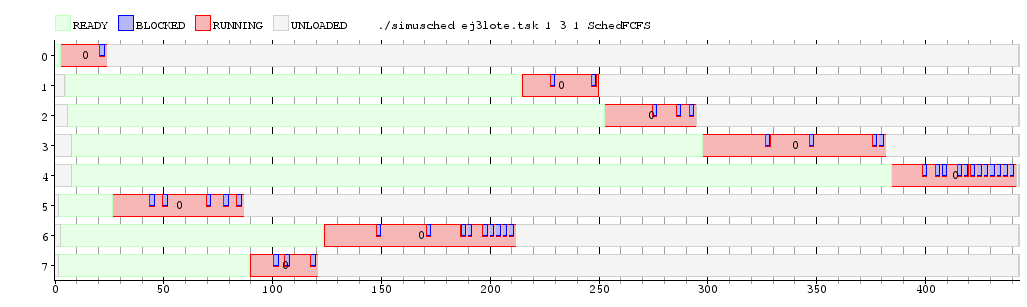
\includegraphics[width=500px]{imagenes/ej3.png}
		\caption{\small{\textbf{Gráfico generado con el lote.}}}
		\label{fig:grafico_ej1}
	\end{center}
\end{figure}

\newpage
\section{Ejercicio 4}

\subsection{Enunciado}
Completar la implementación del scheduler Round-Robin implementando los métodos de la clase \textbf{SchedRR} en los archivos \textbf{sched\_rr.cpp} y \textbf{sched\_rr.h}. La implementación recibe como primer parámetro la cantidad de núcleos y a continuación los valores de sus respectivos quantums. Debe utilizar una única cola global, permitiendo así la migración de procesos entre núcleos.


\subsection{Resolución}

\newpage
\section{Ejercicio 5}

\subsection{Enunciado}
Dado el lote de tareas del ejercicio 2.
~
Ejecutar y graficar la simulación utilizando el scheduler \textit{Round-Robin} con quantum 2, 5 y 10.
Con un cambio de contexto de 2 ciclos y un sólo núcleo calcular la \textit{latencia}, el \textit{waiting time} y el tiempo total de ejecución de las tareas para cada quantum.


\subsection{Resolución}
\newpage
\section{Ejercicio 6}

%El artículo llama nubes o recursos a los servidores, yo a veces me confundo y pongo un nombre u otro, revisar si es confuso
En el paper en cuestión, los autores intentan encontrar un algoritmo de scheduling optimizado para el Cloud Computing. En particular, quieren encontrar un algoritmo que, teniendo en cuenta las singularidades del modelo de Cloud Computing, como lo es el estar orientado a trabajo cooperativo, pero con usuarios con requerimientos diferentes, optimice el tiempo en que cada tarea se encuentra en estado de espera (Ready). En particular, los autores observan como problema que las tareas de alta granularidad pasan gran tiempo en espera.
Los autores analizan los esquemas de scheduling usados en Cloud Computing, en particular Task Grouping y priorización con conciencia de ancho de banda (Prioritization with Bandwidth Awareness). En el primero, consiste en agrupar tareas similares y programarlas en grupo, en particular basándose en el nivel de granularidad, agrupando tareas altamente granulares para simplificar el uso de recursos. En el segundo, el scheduler toma en cuenta el ancho de banda disponible en cada ronda para agrupar y programar las tareas con el objetivo de reducir la latencia de comunicación entre tareas y el tiempo de espera de las mismas.

El algoritmo que proponen los autores se basa en integrar estos dos algoritmos, junto con un Scheduler SJF. Teniendo en cuenta que el agrupamiento tradicional no contempla el ancho de banda de red o el tamaño de los archivos de tarea, el algoritmo propuesto por los autores comienza por la capacidad de procesamiento de cada nube, ordenándolas descendentemente en base a sus MIPS. Luego, con el objetivo de reducir el tiempo de espera de cada tarea, el scheduler agrupa las tareas en base a la granularidad, primero tareas altamente granulares, de acuerdo con la capacidad de procesamiento de la primera nube, y envía la tarea agrupada a la misma, siguiendo de igual forma con las demás.	
En detalle, existen cuatro fases. La primera consta de la inicialización de los recursos y los datos de entrada. Los autores informan que por utilizar la función aleatoria para generar los valores de los mismos (tamaño de archivos, recursos de los servidores, requerimientos de cada tarea) en el momento de la experimentación, cada uno de estos sigue la distribución uniforme. En la segunda fase se ordenan las tareas en base a sus demandas y características y, los recursos en primera instancia según ancho de banda para reducir la latencia de red y en segundo lugar por capacidad de procesamiento. Luego, en la tercera fase se agrupan las tareas y se envían a los servidores ya priorizados como se explicó anteriormente. En cada nube, el grupo de tareas se considera como una sola tarea de baja granularidad y así es ejecutada. En la cuarta y última fase, se aplica un algoritmo SJF en cada servidor para reducir aún más el tiempo de espera de cada tarea.

Para poder analizar el comportamiento del sheduler, los autores decidieron experimentar sobre un simulador (CloudSim) que les permitió modelar todos los servicios necesarios. Se utilizó su set de herramientas para simular los distintos ambientes de ejecución, y los recursos se representaron como parámetros, como lo fuera el ID del recurso, los elementos de procesamiento, MIPS,  ancho de banda y RAM, entre otros. 
En el experimento se utilizaron 10 recursos (servidores) de tiempo compartido y cada uno es alojado en una máquina con características diferentes (en particular, ancho de banda y capacidad de procesamiento, que son los factores que los autores toman para hacer el estudio, todos los servidores tienen 2GB de RAM y el mismo costo por ancho de banda). La capacidad computacional de cada nube se estableció en $200 MIPS \pm 30\%$ .

Cada tarea tiene asociados sus requerimientos de cómputo, el tamaño de los datos de entrada y salida, y otros parámetros. Cada una simula aplicaciones basadas en la nube, como lo es la transferencia de contenido, interacción social, y otras. Para generar las tareas se utilizó una distribución gaussiana con un mínimo de 1 millón de instrucciones y una función aleatoria para generar el tamaño de los archivos de entrada y salida. El tamaño del archivo de tarea y del archivo de salida de la misma se hicieron aleatoriamente en el rango de $100 bytes \pm 30\%$  cada uno, la cantidad de tareas varió de 1000 a 7000 con cambios de a 1000 tareas y la granularidad fue de 10s a 30s con pasos de a 5s.

\newpage
\section{Ejercicio 7}

\subsection{Enunciado}
En base a lo anterior, defina dos nuevos algoritmos de scheduling. Ambos del tipo \textit{shortest job first}. Para ambos puede considerar que solamente correran tareas de tipo TaskCPU.

\begin{enumerate}[a)]
\item Uno no reentrante. Tomará como parámetros la cantidad de procesadores y el tiempo total de ejecución de cada tarea en el lote. Ejecutará la tarea que menos tiempo de cpu necesite. Al terminar de ejecutarla, volverá a elegir la de menor tiempo de ejecución.
Será llamado \textbf{SJF}.

\item Uno reentrante. Tomará como parámetros la cantidad de procesadores, los \textbf{Quantums} de cada uno de ellos y el tiempo total de ejecución de cada tarea en el lote. Un proceso correrá en ese procesador durante ese quantum. Al terminar dicho tiempo, ejecutará la tarea a la que menos tiempo le quede de ejecución (podría seguir ejecutando la tarea actual). Existe una única cola de procesos para todos los procesadores. Lo llamaremos
\textbf{RSJF}.
\end{enumerate}

\subsection{Resolución}

Para este ejercicio se pedía realizar las implementaciones de dos nuevos algoritmos de scheduling, del tipo \emph{shortest job first}, que sólo corren tareas del tipo TaskCPU.
La primera de ellas, llamada \textbf{SJF}, elige y ejecuta siempre la tarea con el menor tiempo de CPU que necesite hasta terminar.
La segunda, llamada \textbf{RSJF}, también elige y ejectua la tarea con el menor tiempo de CPU que necesite pero, cada core posée un quantum por lo que cuando se termina éste, se toma una nueva tarea con el menor tiempo de CPU, se encola la tarea desalojada y luego se reinicia el quantum del core.

\subsection{Implementación \textbf{SJF}}

Esta implementación toma como parametros la cantidad de cores y los tiempos de cada proceso a ser ejecutado en el orden en que se los carga.

Para facilitar el manejo de los procesos con sus respectivos tiempos, generamos un struct llamada \emph{Proceso} que tiene como estructura el pid del proceso y su tiempo de ejecución. También posée el operador $<$ que sirve para comparar los tiempos de los procesos.

Con esto, el scheduler posée como estructra dos colas:

\begin{itemize}

\item \emph{tiempos\_procesos}: una cola normal que se utiliza para encolar los tiempos de los procesos que recibe como parametro este scheduler.

\item \emph{cola\_procesos}: esta es una cola de prioridad de la estructura Proceso, donde la máxima prioridad la tiene el proceso con menor tiempo de ejecución.

\end{itemize}

El constructor de este scheduler simplemente encola los tiempos de los procesos en la cola \emph{tiempos\_procesos}.

La función \textbf{load} crea un nuevo Proceso con el pid que recibe como parametro y el primer elemento de la cola (ya que ésta tiene los tiempos de los elementos en el orden que van llegando) y encolo este Proceso en la cola de prioridad \emph{cola\_procesos}.

La función \textbf{unblock} no se utiliza ya que, por enunciado, este scheduler sólo corre tareas del tipo TaskCPU (que no tiene llamadas bloqueantes).

La función \textbf{tick} en este scheduler es muy sencilla, pasamos a mostrar un pseudocódigo que muestre su comportamiento:

\begin{algorithmic}
\Function{int tick}{int cpu, const enum Motivo m}

	\If {\emph{(Si la tarea actual es la IDLE\_TASK o el motivo es que terminó el proceso actual) y la cola de prioridad \textbf{cola\_procesos} no está vacía}}
		\State Desencolo de \textbf{cola\_procesos} el primero elemento (o sea, el que tiene el menor tiempo) y lo devuelvo.
	
	\ElsIf{\emph{Si el motivo es que pasó un tick de reloj}}
		\State Devuelvo el proceso actual.

	\Else
		\State Devuelvo IDLE\_TASK.
	\EndIf
\EndFunction	
\end{algorithmic}


\subsection{Implementación \textbf{RSJF}}


\newpage
\section{Ejercicio 8}

\subsection{Enunciado}
Resuelva:

\begin{enumerate}[a)]
\item Realice tareas de prueba para comparar los schedulers \textbf{Round Robin}, \textbf{FIFO}, \textbf{SJF}, \textbf{RSJF}.

\item Compárelas según la \textbf{latencia}, \textbf{waiting time}, \textbf{turnaround}.
\newline
Realice gráficos y tablas comparativas para exponer los resultados obtenidos.

\item Escriba una breve conclusión.

\end{enumerate}


\subsection{Resolución}

Para este ejercicio se pedía realizar tareas de prueba para comparar los scheduleres \emph{Round Robin}, \emph{FCFS}, \emph{SJF} y \emph{RSJF}.

Luego, realizar comparaciones según latencia, waiting time y turnaround, realizar gráficos y tablas para exponer los resultados y dar una conclusión.

Como los schedulers \emph{SJF} y \emph{RSJF} sólo toman tareas del tipo TaskCPU, los lotes generados para los experimentos son con este tipo de tareas.

También, en los experimentos el costo de cambiar de contexto es de dos y el costo de cambiar un proceso de núcleo es de uno.

\subsection{Primera Prueba}

Para esta prueba utilizamos el lote de tareas \textbf{ej8lote1}, en donde estas son lanzadas en al mismo tiempo al comienzo de la ejecución. Los tiempos tomados para ellas son 5, 7, 3, 11 y 2.

La cantidad de cores utilizados en este caso es de uno. Y, en el caso de \emph{Round Robin} y \emph{RSJF}, el quantum dado es 3.

Lo que intentamos ver en esta prueba es, dado este lote de tareas, el comportamiento, velocidad en ejecutar y terminar estas con los schedulers implementados.

Los gráficos obtenidos son:

\begin{figure}[!h]
	\begin{center}
		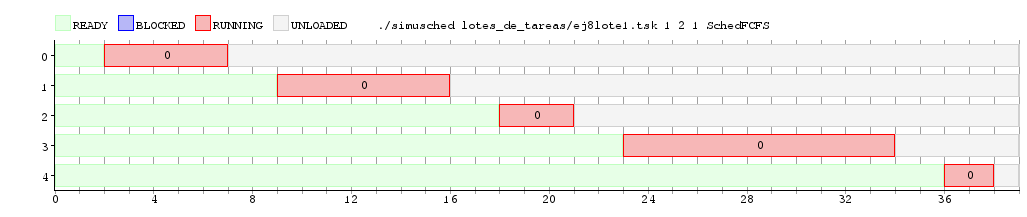
\includegraphics[width=500px]{imagenes/ej8_prueba1_fcfs.png}
		\caption{Ejecución del lote \emph{ej8lote1} con scheduler FCFS.}
		\label{fig:grafico_ej8_prueba1_fcfs}
	\end{center}
\end{figure}

\begin{figure}[!h]
	\begin{center}
		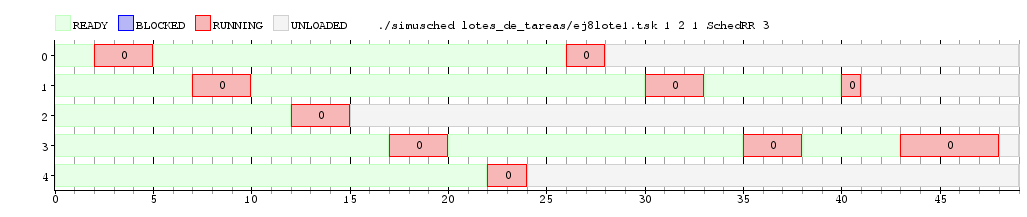
\includegraphics[width=500px]{imagenes/ej8_prueba1_rr.png}
		\caption{Ejecución del lote \emph{ej8lote1} con scheduler Round Robin.}
		\label{fig:grafico_ej8_prueba1_rr}
	\end{center}
\end{figure}

\begin{figure}[!h]
	\begin{center}
		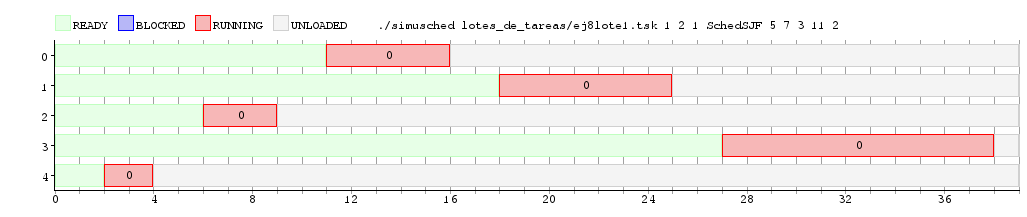
\includegraphics[width=500px]{imagenes/ej8_prueba1_sjf.png}
		\caption{Ejecución del lote \emph{ej8lote1} con scheduler SJF.}
		\label{fig:grafico_ej8_prueba1_sjf}
	\end{center}
\end{figure}

\begin{figure}[!h]
	\begin{center}
		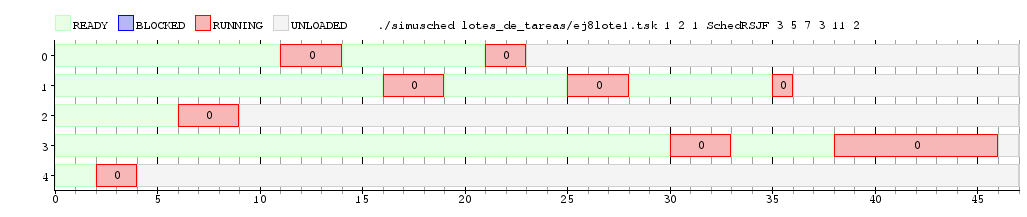
\includegraphics[width=500px]{imagenes/ej8_prueba1_rsjf.png}
		\caption{Ejecución del lote \emph{ej8lote1} con scheduler RSJF.}
		\label{fig:grafico_ej8_prueba1_rsjf}
	\end{center}
\end{figure}

%LATENCIA PROMEDIO
\begin{center}
	\begin{tabular}{|c|c|c|c|}
		\hline
		\multicolumn{4}{|c|}{\large{\textbf{Latencia Promedio}}} \\
		\hline
		\textbf{FCFS} & \textbf{Round Robin} & \textbf{SJF} & \textbf{RSJF} \\
		\hline
		17,6 & 12 & 12,8 & 13 \\
		\hline
	\end{tabular}
\end{center}

%WAITING TIME PROMEDIO
\begin{center}
	\begin{tabular}{|c|c|c|c|}
		\hline
		\multicolumn{4}{|c|}{\large{\textbf{Waiting Time Promedio}}} \\
		\hline
		\textbf{FCFS} & \textbf{Round Robin} & \textbf{SJF} & \textbf{RSJF} \\
		\hline
		17,6 & 25,6 & 12,8 & 18 \\
		\hline
	\end{tabular}
\end{center}

%TIEMPO TOTAL DE EJECUCION PROMEDIO
\begin{center}
	\begin{tabular}{|c|c|c|c|}
		\hline
		\multicolumn{4}{|c|}{\large{\textbf{Tiempo Total De Ejecución Promedio}}} \\
		\hline
		\textbf{FCFS} & \textbf{Round Robin} & \textbf{SJF} & \textbf{RSJF} \\
		\hline
		23,2 & 31,2 & 18,4 & 23,6 \\
		\hline
	\end{tabular}
\end{center}

BREVE COMENTARIO SOBRE DATOS OBTENIDOS

AHORA CON DOS CORES (QUANTUM 3 PARA CADA UNO PARA RR Y RSJF)

\begin{figure}[!h]
	\begin{center}
		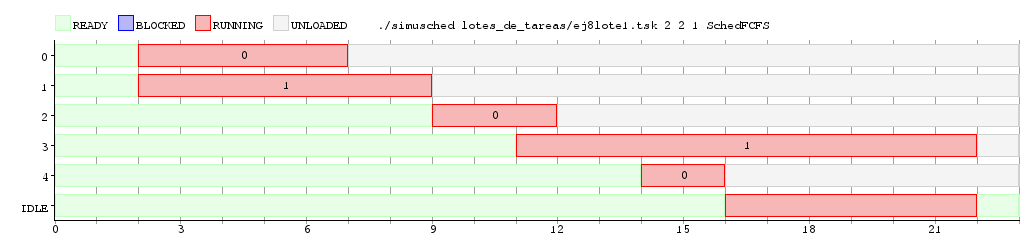
\includegraphics[width=500px]{imagenes/ej8_prueba1_fcfs2.png}
		\caption{Ejecución del lote \emph{ej8lote1} con scheduler FCFS con 2 cores.}
		\label{fig:grafico_ej8_prueba1_fcfs2}
	\end{center}
\end{figure}

\newpage

\begin{figure}[!h]
	\begin{center}
		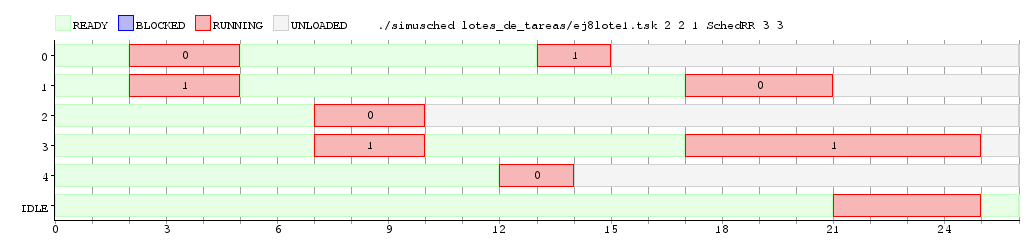
\includegraphics[width=500px]{imagenes/ej8_prueba1_rr2.png}
		\caption{Ejecución del lote \emph{ej8lote1} con scheduler Round Robin con dos cores.}
		\label{fig:grafico_ej8_prueba1_rr2}
	\end{center}
\end{figure}

\begin{figure}[!h]
	\begin{center}
		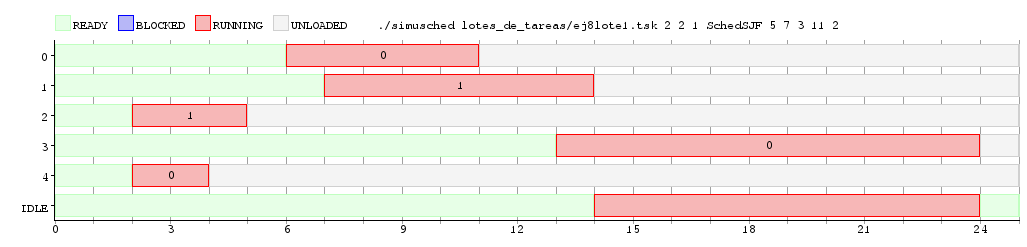
\includegraphics[width=500px]{imagenes/ej8_prueba1_sjf2.png}
		\caption{Ejecución del lote \emph{ej8lote1} con scheduler SJF con dos cores.}
		\label{fig:grafico_ej8_prueba1_sjf2}
	\end{center}
\end{figure}

\begin{figure}[!h]
	\begin{center}
		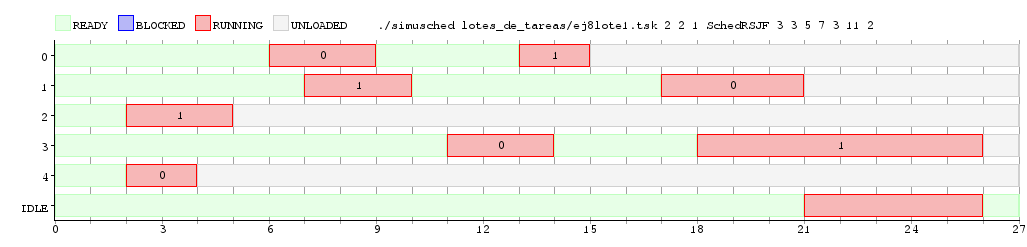
\includegraphics[width=500px]{imagenes/ej8_prueba1_rsjf2.png}
		\caption{Ejecución del lote \emph{ej8lote1} con scheduler RSJF con dos cores.}
		\label{fig:grafico_ej8_prueba1_rsjf2}
	\end{center}
\end{figure}

%LATENCIA PROMEDIO
\begin{center}
	\begin{tabular}{|c|c|c|c|}
		\hline
		\multicolumn{4}{|c|}{\large{\textbf{Latencia Promedio}}} \\
		\hline
		\textbf{FCFS} & \textbf{Round Robin} & \textbf{SJF} & \textbf{RSJF} \\
		\hline
		7,6 & 6 & 6 & 5,6 \\
		\hline
	\end{tabular}
\end{center}

%WAITING TIME PROMEDIO
\begin{center}
	\begin{tabular}{|c|c|c|c|}
		\hline
		\multicolumn{4}{|c|}{\large{\textbf{Waiting Time Promedio}}} \\
		\hline
		\textbf{FCFS} & \textbf{Round Robin} & \textbf{SJF} & \textbf{RSJF} \\
		\hline
		17,6 & 11,4 & 6 & 8,6 \\
		\hline
	\end{tabular}
\end{center}

%TIEMPO TOTAL DE EJECUCION PROMEDIO
\begin{center}
	\begin{tabular}{|c|c|c|c|}
		\hline
		\multicolumn{4}{|c|}{\large{\textbf{Tiempo Total De Ejecución Promedio}}} \\
		\hline
		\textbf{FCFS} & \textbf{Round Robin} & \textbf{SJF} & \textbf{RSJF} \\
		\hline
		17,6 & 17 & 11,6 & 14,2 \\
		\hline
	\end{tabular}
\end{center}

BREVE COMENTARIO SOBRE MEJORAS

\subsection{Segunda Prueba}

Para esta prueba utilizamos el lote de tareas \textbf{ej8lote1}, en donde estas son lanzadas con una diferencia de dos ticks desde el comienzo de la ejecución. Los tiempos tomados para ellas son los mismos que los utilizados la prueba anterior.

En esta prueba, como la anterior, comenzamos utilizando un core por scheduler y, para los schedulers \emph{Round Robin} y \emph{RSJF}, el quantum dado es 3.

La cantidad de cores utilizados en este caso es de uno. Y, en el caso de \emph{Round Robin} y \emph{RSJF}, el quantum dado es 3.

En este caso, intentamos ver el comportamiento de los schedulers en donde las tareas van apareciendo con una frecuencia constante.

Los graficos obtenidos son:

\begin{figure}[!h]
	\begin{center}
		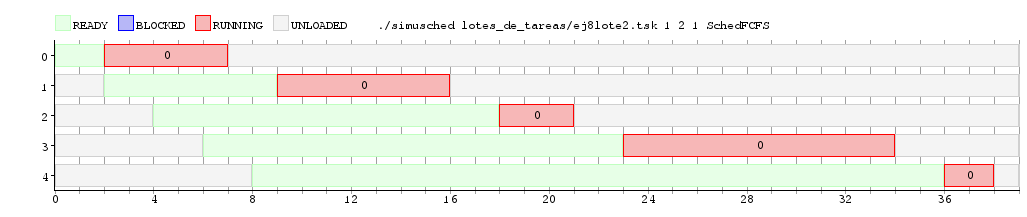
\includegraphics[width=500px]{imagenes/ej8_prueba2_fcfs.png}
		\caption{Ejecución del lote \emph{ej8lote2} con scheduler FCFS.}
		\label{fig:grafico_ej8_prueba2_fcfs}
	\end{center}
\end{figure}

\begin{figure}[!h]
	\begin{center}
		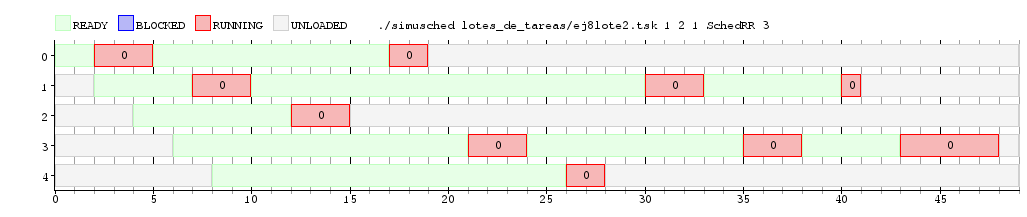
\includegraphics[width=500px]{imagenes/ej8_prueba2_rr.png}
		\caption{Ejecución del lote \emph{ej8lote2} con scheduler Round Robin.}
		\label{fig:grafico_ej8_prueba2_rr}
	\end{center}
\end{figure}

\begin{figure}[!h]
	\begin{center}
		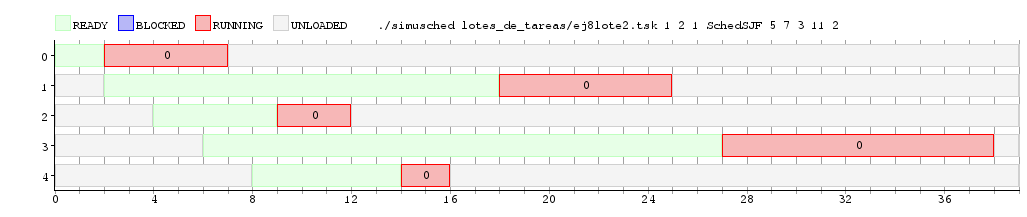
\includegraphics[width=500px]{imagenes/ej8_prueba2_sjf.png}
		\caption{Ejecución del lote \emph{ej8lote2} con scheduler SJF.}
		\label{fig:grafico_ej8_prueba2_sjf}
	\end{center}
\end{figure}

\newpage

\begin{figure}[!h]
	\begin{center}
		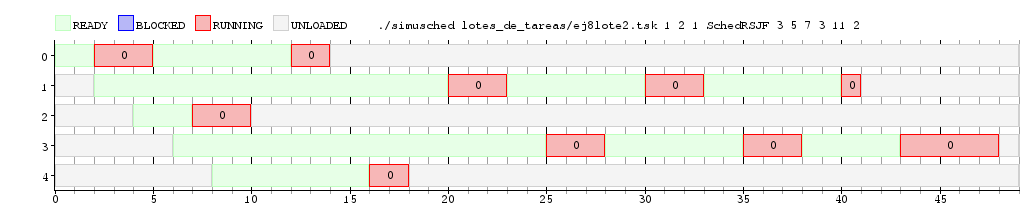
\includegraphics[width=500px]{imagenes/ej8_prueba2_rsjf.png}
		\caption{Ejecución del lote \emph{ej8lote2} con scheduler RSJF.}
		\label{fig:grafico_ej8_prueba2_rsjf}
	\end{center}
\end{figure}

%LATENCIA PROMEDIO
\begin{center}
	\begin{tabular}{|c|c|c|c|}
		\hline
		\multicolumn{4}{|c|}{\large{\textbf{Latencia Promedio}}} \\
		\hline
		\textbf{FCFS} & \textbf{Round Robin} & \textbf{SJF} & \textbf{RSJF} \\
		\hline
		11,2 & 6 & 8,8 & 8,4 \\
		\hline
	\end{tabular}
\end{center}

%WAITING TIME PROMEDIO
\begin{center}
	\begin{tabular}{|c|c|c|c|}
		\hline
		\multicolumn{4}{|c|}{\large{\textbf{Waiting Time Promedio}}} \\
		\hline
		\textbf{FCFS} & \textbf{Round Robin} & \textbf{SJF} & \textbf{RSJF} \\
		\hline
		11,2 & 20,6 & 14,8 & 13 \\
		\hline
	\end{tabular}
\end{center}

%TIEMPO TOTAL DE EJECUCION PROMEDIO
\begin{center}
	\begin{tabular}{|c|c|c|c|}
		\hline
		\multicolumn{4}{|c|}{\large{\textbf{Tiempo Total De Ejecución Promedio}}} \\
		\hline
		\textbf{FCFS} & \textbf{Round Robin} & \textbf{SJF} & \textbf{RSJF} \\
		\hline
		17,6 & 20,6 & 10 & 16,6 \\
		\hline
	\end{tabular}
\end{center}

BREVE COMENTARIO SOBRE DATOS OBTENIDOS

AHORA CON DOS CORES (QUANTUM 3 PARA CADA UNO PARA RR Y RSJF)

\begin{figure}[!h]
	\begin{center}
		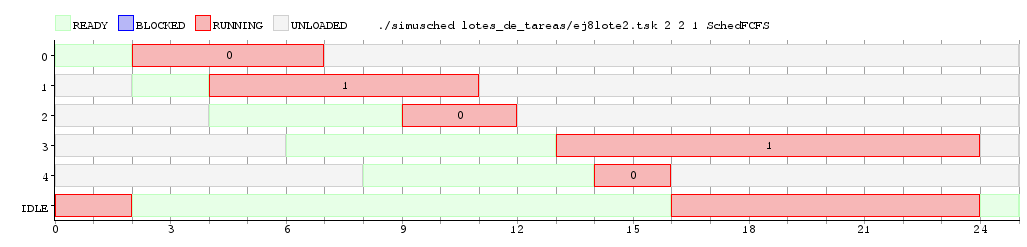
\includegraphics[width=500px]{imagenes/ej8_prueba2_fcfs2.png}
		\caption{Ejecución del lote \emph{ej8lote2} con scheduler FCFS con 2 cores.}
		\label{fig:grafico_ej8_prueba2_fcfs2}
	\end{center}
\end{figure}

\begin{figure}[!h]
	\begin{center}
		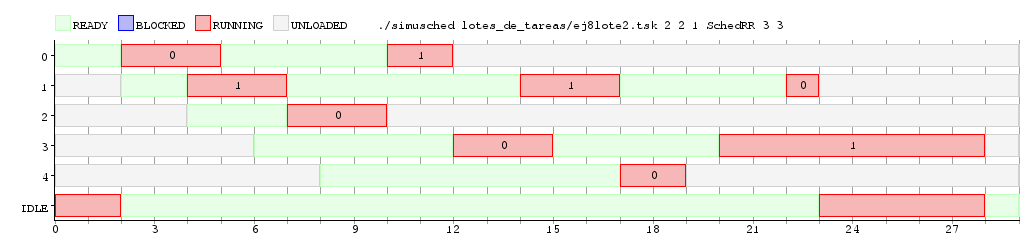
\includegraphics[width=500px]{imagenes/ej8_prueba2_rr2.png}
		\caption{Ejecución del lote \emph{ej8lote2} con scheduler Round Robin con dos cores.}
		\label{fig:grafico_ej8_prueba2_rr2}
	\end{center}
\end{figure}

\newpage

\begin{figure}[!h]
	\begin{center}
		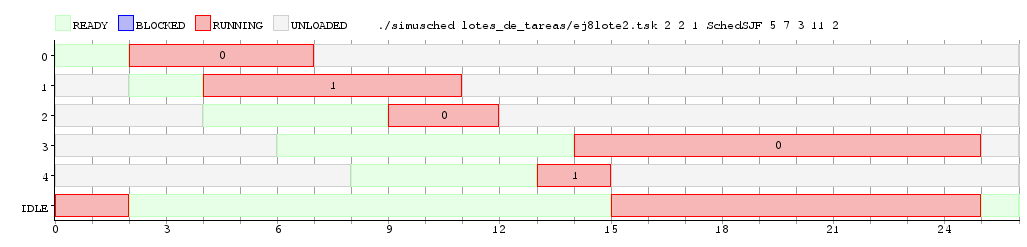
\includegraphics[width=500px]{imagenes/ej8_prueba2_sjf2.png}
		\caption{Ejecución del lote \emph{ej8lote2} con scheduler SJF con dos cores.}
		\label{fig:grafico_ej8_prueba2_sjf2}
	\end{center}
\end{figure}

\begin{figure}[!h]
	\begin{center}
		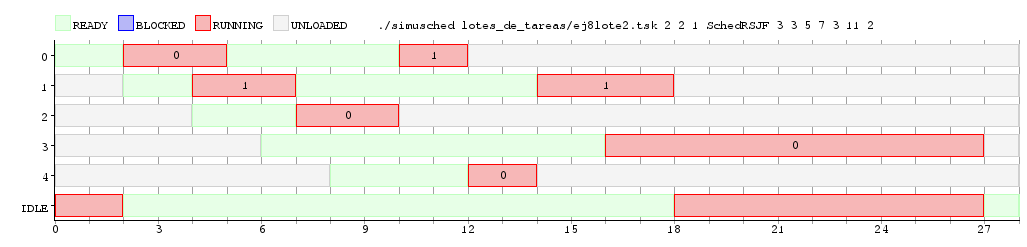
\includegraphics[width=500px]{imagenes/ej8_prueba2_rsjf2.png}
		\caption{Ejecución del lote \emph{ej8lote2} con scheduler RSJF con dos cores.}
		\label{fig:grafico_ej8_prueba2_rsjf2}
	\end{center}
\end{figure}

%LATENCIA PROMEDIO
\begin{center}
	\begin{tabular}{|c|c|c|c|}
		\hline
		\multicolumn{4}{|c|}{\large{\textbf{Latencia Promedio}}} \\
		\hline
		\textbf{FCFS} & \textbf{Round Robin} & \textbf{SJF} & \textbf{RSJF} \\
		\hline
		4,4 & 4,4 & 4,4 & 4,2 \\
		\hline
	\end{tabular}
\end{center}

%WAITING TIME PROMEDIO
\begin{center}
	\begin{tabular}{|c|c|c|c|}
		\hline
		\multicolumn{4}{|c|}{\large{\textbf{Waiting Time Promedio}}} \\
		\hline
		\textbf{FCFS} & \textbf{Round Robin} & \textbf{SJF} & \textbf{RSJF} \\
		\hline
		4,4 & 8,8 & 4,4 & 6,6 \\
		\hline
	\end{tabular}
\end{center}

%TIEMPO TOTAL DE EJECUCION PROMEDIO
\begin{center}
	\begin{tabular}{|c|c|c|c|}
		\hline
		\multicolumn{4}{|c|}{\large{\textbf{Tiempo Total De Ejecución Promedio}}} \\
		\hline
		\textbf{FCFS} & \textbf{Round Robin} & \textbf{SJF} & \textbf{RSJF} \\
		\hline
		10 & 14,4 & 10 & 12,2 \\
		\hline
	\end{tabular}
\end{center}

BREVE COMENTARIO SOBRE MEJORAS

\newpage
\section{Ejercicio 9}

\subsection{Enunciado}
Completar la implementación del scheduler \textit{Multilevel Feedback Queue} implementando los métodos de la clase \textbf{SchedMFQ} en los archivos \textbf{sched\_mfq.cpp} y \textbf{sched\_mfq.h}.
La implementación debe utilizar \textit{n} colas con \textit{Round-Robin} en cada una con los parámetros que se detallan a continuación.

\begin{itemize}
\item Las n colas se numeran de 0 a $n-1$ siendo 0 la de mayor prioridad.

\item El constructor recibe como parámetro $n$ números $q_i$ indicando el \textit{quantum} de la cola $i$.

\item Al iniciar una tarea comienza al final de la cola de mayor prioridad.

\item Siempre se ejecuta la primer tarea de la cola no vacía de mayor prioridad. Si esta tarea consume todo su \textit{quantum} sin bloquearse entonces pasa al final de la cola inmediatamente de inferior prioridad (si hay). Si esta tarea se bloquea antes de agotar su \textit{quantum}, entonces (cuando se desbloquee)

\item Si todas las colas están vacías se ejecuta \textbf{IDLE TASK}.

\end{itemize}

Realice pruebas y muestre su ejecución.

\subsection{Resolución}

\end{document}
